我们提出的方法的概述如图\ref{fig:pipeline}所示。我们的方法以点对应关系作为输入。接着通过检查对应关系之间的距离一致性来构建一个不变性一致性矩阵。然后,通过将列或行向量视为这些对应关系的“特征”,将这些对应关系快速聚类成不同的组。通过凝聚聚类方法高效地进行聚类,然后通过交替合并相似的变换和重新分配簇标签进行多次迭代来进一步优化。在对应关系数量较大的情况下,我们可以选择性地应用降采样和上采样过程。详细内容将在接下来的章节中介绍。

\begin{figure*}[ht]
    \centering
    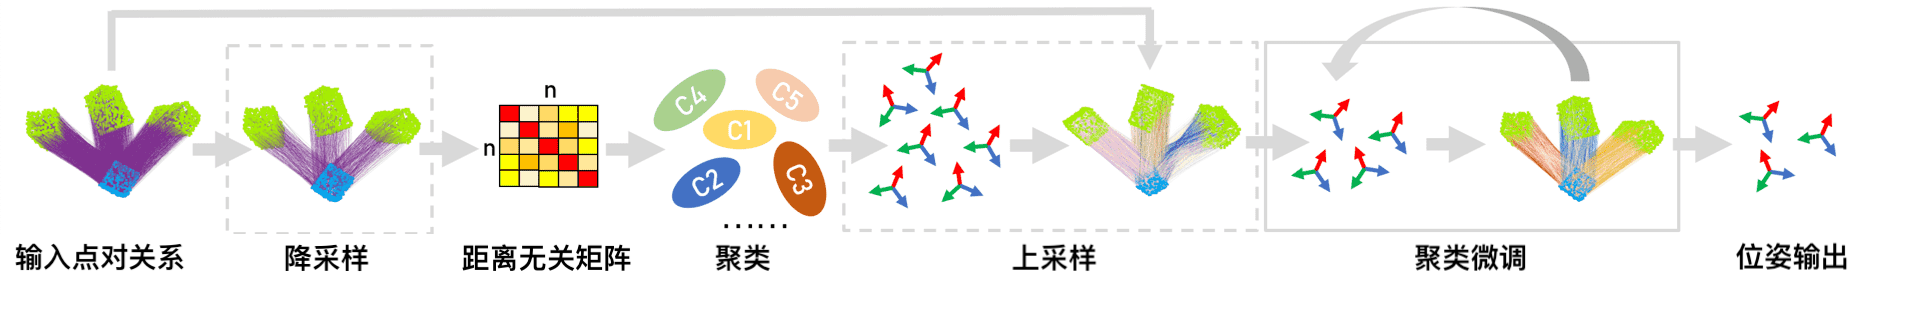
\includegraphics[width=1\textwidth]{images/pipeline.png} % Reduce the figure size so that it is slightly narrower than the column. Don't use precise values for figure width.This setup will avoid overfull boxes.
    \caption{我们提出的多实例点云配准方法的流程。从输入对应关系构建距离不变性矩阵,用于将对应关系聚类为不同的簇(\textbf{聚类}),并进行优化(\textbf{簇优化})。最后,从每个对应关系簇中估计与每个实例相关的刚体变换(\textbf{变换})。为了处理大量的对应关系,采用两个附加过程(\textbf{下采样}和\textbf{上采样})。}
    \label{fig:pipeline}
    \vspace{-0.6in}
\end{figure*}

\section{不变性矩阵和兼容性向量}
\label{subsec:Distance-Consistency-Graph}
距离不变性特性在3D配准领域已经被研究多年\cite{TEASER}\cite{shi2021robin}\cite{leordeanu2005spectral},该特性描述了在刚性变换之后两点之间的距离保持不变。具体来说,如果 $c_i :\mathbf{x}i \leftrightarrow \mathbf{y}i$ 和 $c_j : \mathbf{x}j \leftrightarrow \mathbf{y}j$ 是两个真实的对应关系,那么它们应该满足
%
\begin{equation}
G{ij}=|d{ij} - d'{ij} | < \delta
\label{eq:abs_diff}
\end{equation}
其中 $d{ij} = |\mathbf{x}i-\mathbf{x}j|, d'{ij}=|\mathbf{y}i -\mathbf{y}j|$,$\delta $ 是一个用于考虑噪声的阈值。
因此,$d{ij}$ 和 $d'{ij}$ 之间的差异可以用作度量是否存在异常值,或者两个对应关系是否来自不同的刚性变换的指标。我们参考\cite{matrix},使用相对差异作为度量,而不是在(\ref{eq:abs_diff})中定义的绝对差异,
\begin{equation}
G{ij} = s_{ij}^2, s_{ij} = \min( \frac{d_{ij}}{d'{ij}}, \frac{d'{ij}}{d_{ij}}) \in (0, 1).
\end{equation}
通过计算所有对应关系对之间的分数,可以获得一个\emph{距离不变性矩阵} $G$(我们令 $G_{ii} = 1$)。距离不变性矩阵是对称的,其中每一列或行是一个向量,描述了给定对应关系与其他对应关系之间的兼容性\cite{reviewof3dourlierremovingjiaqiYang}。